% ==============================================================================
% 第 28 章：数学实例 (Chapter 28: Mathematical Examples)
% ==============================================================================

\chapter{数学实例}
\label{sec:ch28_math}

许多数学问题的计算机求解都深刻依赖于生成型递归。未来的软件工程师必须熟练掌握这些经典解法，其原因有二：一方面，相当一部分实际编程任务本质上就是将这类数学思想转化为高效程序；另一方面，在数学问题上的思维训练往往能为算法设计提供极具启发性的灵感源泉。本章将深入研讨三个此类核心经典问题：牛顿求根法、数值积分以及高斯消元法。

\section{牛顿法}
\label{sec:28_1}

第 27.2 节介绍了寻找数学函数零点的一种方法（二分法）。在纯粹的数学与科学计算领域，程序员更倾向于采用源自微积分分析的高效方法，其中最著名的当属\term{牛顿法（Newton's method）}。与二分法类似，牛顿法通过反复迭代来逐步改进对零点的近似值，直至足够逼近目标。

从一个初始猜测值 $r_1$ 出发，牛顿法的核心计算过程在于：\textbf{构造函数 $f$ 在点 $r_1$ 处的切线（tangent），并求解该切线的零点}。由于切线在局部线性逼近了原函数，而求解一条直线的零点极为简便，通过充分多次重复该迭代过程，算法通常能够迅速收敛到一个使得 $f(r)$ 极其接近 0 的精确数值 $r$。

显然，这一过程依赖于有关切线的两项数学领域知识：其斜率与零点。直观上，函数 $f$ 在点 $r_1$ 处的切线是穿过点 $(r_1, f(r_1))$ 且与曲线 $f$ 具有相同斜率的直线。在数值计算中，获取切线斜率的一种标准方式是在 $x$ 轴上选取关于 $r_1$ 对称的两个微小间距点：$r_1 - \varepsilon$ 与 $r_1 + \varepsilon$（其中 $\varepsilon$ 是一个充分小的正常数）。由两点 $(r_1 - \varepsilon, f(r_1 - \varepsilon))$ 和 $(r_1 + \varepsilon, f(r_1 + \varepsilon))$ 确定的割线斜率即可作为切线斜率的高精度近似：
\[ \text{slope} = \frac{f(r_1 + \varepsilon) - f(r_1 - \varepsilon)}{2\varepsilon} \]

\begin{exercise}{数值导数与斜率函数 slope}{455}\label{ex:455}
将上述数学公式翻译为 ISL+ 函数 \code{slope}。它接收函数 $f$ 与数值 $r_1$，输出 $f$ 在 $r_1$ 处的数值斜率。假设 $\varepsilon$ 为全局常量。编写测试用例验证水平线、线性函数以及简单多项式的斜率计算。
\end{exercise}

第二项领域知识是切线的零点。切线本身是一条直线（线性函数），它经过点 $(r_1, f(r_1))$ 且具有斜率 $m = \text{slope}$。在数学上，其方程可表示为：
\[ \text{tangent}(x) = f(r_1) + m \cdot (x - r_1) \]
寻找切线的零点即求解方程 $\text{tangent}(\text{root-of-tangent}) = 0$：
\[ f(r_1) + m \cdot (\text{root-of-tangent} - r_1) = 0 \]
直接求解该一元一次方程可得：
\[ \text{root-of-tangent} = r_1 - \frac{f(r_1)}{m} \]

\begin{exercise}{切线零点函数 root-of-tangent}{456}\label{ex:456}
设计函数 \code{root-of-tangent}，它接收函数 $f$ 与数值 $r_1$，计算通过点 $(r_1, f(r_1))$ 的切线的零点。
\end{exercise}

现在依照生成型递归的设计配方来实现牛顿法。函数 \code{newton} 接收待求根函数 $f$ 与初始猜测 $r_1$：

\begin{lstlisting}[language=BSL]
; [Number -> Number] Number -> Number
; 寻找数值 r 使得 (f r) 接近 0
; 生成型递归：反复生成改进后的猜测值
(define (newton f r1) 1.0)
\end{lstlisting}

回答四个核心设计问题：
\begin{enumerate}
  \item \textbf{平凡情形判断}：当 $|f(r_1)| \le \varepsilon$ 时，当前猜测已足够精确，问题已解。
  \item \textbf{平凡解}：直接返回 $r_1$。
  \item \textbf{生成子问题}：计算 $f$ 在 $r_1$ 处切线的零点作为下一次更优的猜测值，即 \code{(root-of-tangent f r1)}，并以该新值递归调用 \code{newton}。
  \item \textbf{合并解}：递归子问题的解直接就是原问题的解。
\end{enumerate}

图~\ref{fig:newton-code} 展示了 \code{newton} 的完整实现。

\begin{figure}[htbp]
  \centering
\begin{lstlisting}[language=BSL]
; [Number -> Number] Number -> Number
; 寻找数值 r 使得 (<= (abs (f r)) ε)
(check-within (newton poly 1) 2 ε)
(check-within (newton poly 3.5) 4 ε)

(define (newton f r1)
  (cond
    [(<= (abs (f r1)) ε) r1]
    [else (newton f (root-of-tangent f r1))]))
\end{lstlisting}
  \caption{牛顿法求根程序}
  \label{fig:newton-code}
\end{figure}

此时设计并未结束。配方的第七步要求深入剖析牛顿法的停机性。对于如下二次多项式：
\begin{lstlisting}[language=BSL]
; Number -> Number
(define (poly x) (* (- x 2) (- x 4)))
\end{lstlisting}
其真根为 2 和 4。图~\ref{fig:poly-graph} 展示了 \code{poly} 的曲线：它在对称轴 $x = 3$ 处达到极小值，切线完全水平（斜率为 0）。

\begin{figure}[htbp]
  \centering
  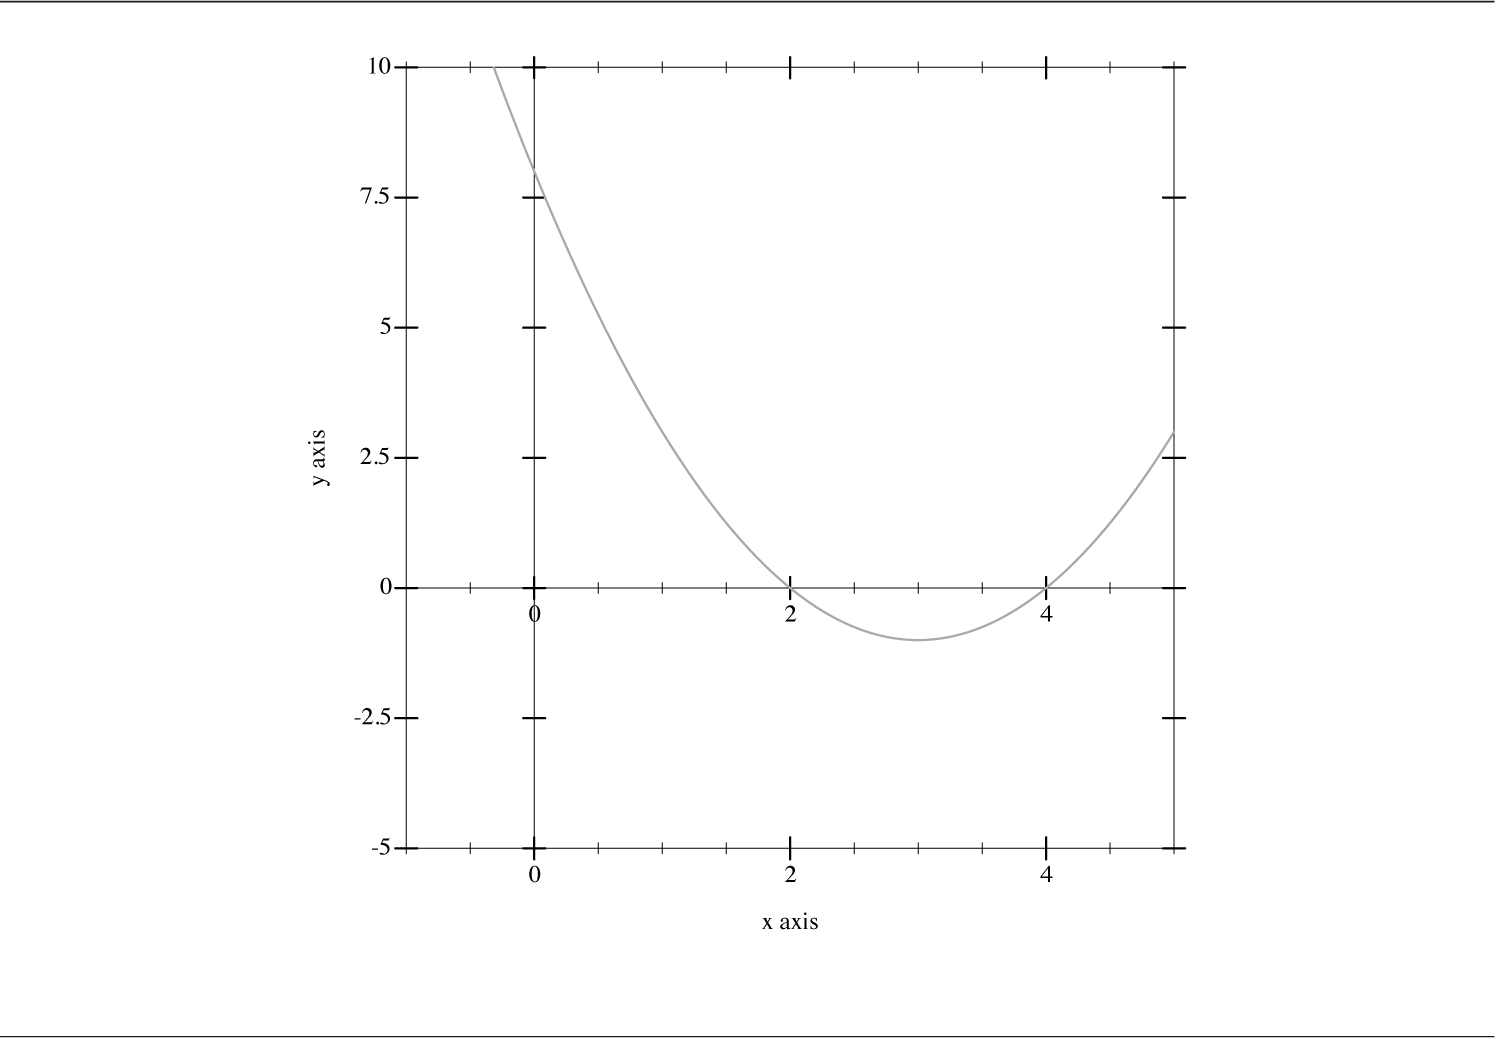
\includegraphics[width=0.75\textwidth]{images/00623.png}
  \caption{\code{poly} 在区间 $[-1, 5]$ 上的图像}
  \label{fig:poly-graph}
\end{figure}

如果以 3 作为初始猜测调用 \code{newton}，计算将会崩溃：
\begin{lstlisting}[language=BSL]
> (poly 3)
-1
> (newton poly 3)
/: division by zero
\end{lstlisting}
原因在于此时切线斜率为 0，除以斜率引发了除零异常。

除了除零错误之外，牛顿法还暴露了与数值精度相关的另外两个严峻停机性问题：
\begin{itemize}
  \item \textbf{精确有理数运算导致的假性“挂起”}：如果在 DrRacket 中传入精确浮点数 \code{2.9999}，ISL+ 会将其作为精确有理分数（如 $29999/10000$）进行无损分数算术。随着连续求导与分式计算，分母与分子的位宽会以指数级爆炸膨胀，导致运算速度急剧下降，耗费数分钟甚至让人误以为程序已经陷入死循环。
  \item \textbf{不精确浮点数导致的发散死循环}：若传入不精确数 \code{\#i3.0}，由于浮点除零会产生 \code{\#i+inf.0}（无穷大），进而参与后续运算产生 \code{\#i+nan.0}（非数），程序将彻底跌入无限递归死循环。
\end{itemize}

因此，编写科学计算函数时，必须在文档和函数头中极为审慎地注明这些收敛陷阱与停机前置条件。

\begin{exercise}{72 法则与资金翻倍计算}{457}\label{ex:457}
设计函数 \code{double-amount}，计算当储蓄账户按月以固定月利率计息时，一笔本金翻倍所需经历的月数。通过代数化简证明本金具体数额无关紧要，仅利率起决定性作用；并验证金融学中著名的“72 法则”（即翻倍月数约为 $72/r$）。
\end{exercise}

\section{数值积分}
\label{sec:28_2}

诸多物理学与工程问题的本质都可归结为计算曲线下方的面积：
\begin{notebox}[物理样例问题]
一辆汽车以恒定速度 $v$ 米/秒行驶，在 5 秒、10 秒、15 秒后行驶的位移是多少？一架火箭以恒定加速度 $a = 12\text{ m/s}^2$ 垂直发射升空，在 5 秒、10 秒、15 秒后达到的高度是多少？
\end{notebox}

物理学定律表明，匀速运动的位移等于矩形面积 $d_{\text{con}}(t) = v \cdot t$；而匀加速运动的位移则对应于三角形面积 $d_{\text{acc}}(t) = \frac{1}{2} a \cdot t^2$。在更广泛的物理世界中，物体在一段时间内运动的位移，严格对应于其速度函数曲线与时间轴之间所围成的曲边梯形面积，如图~\ref{fig:motion-integral} 所示。在给定区间内确定函数图像下方所围面积的计算过程被称为\term{数值积分（numeric integration）}。

\begin{figure}[htbp]
  \centering
  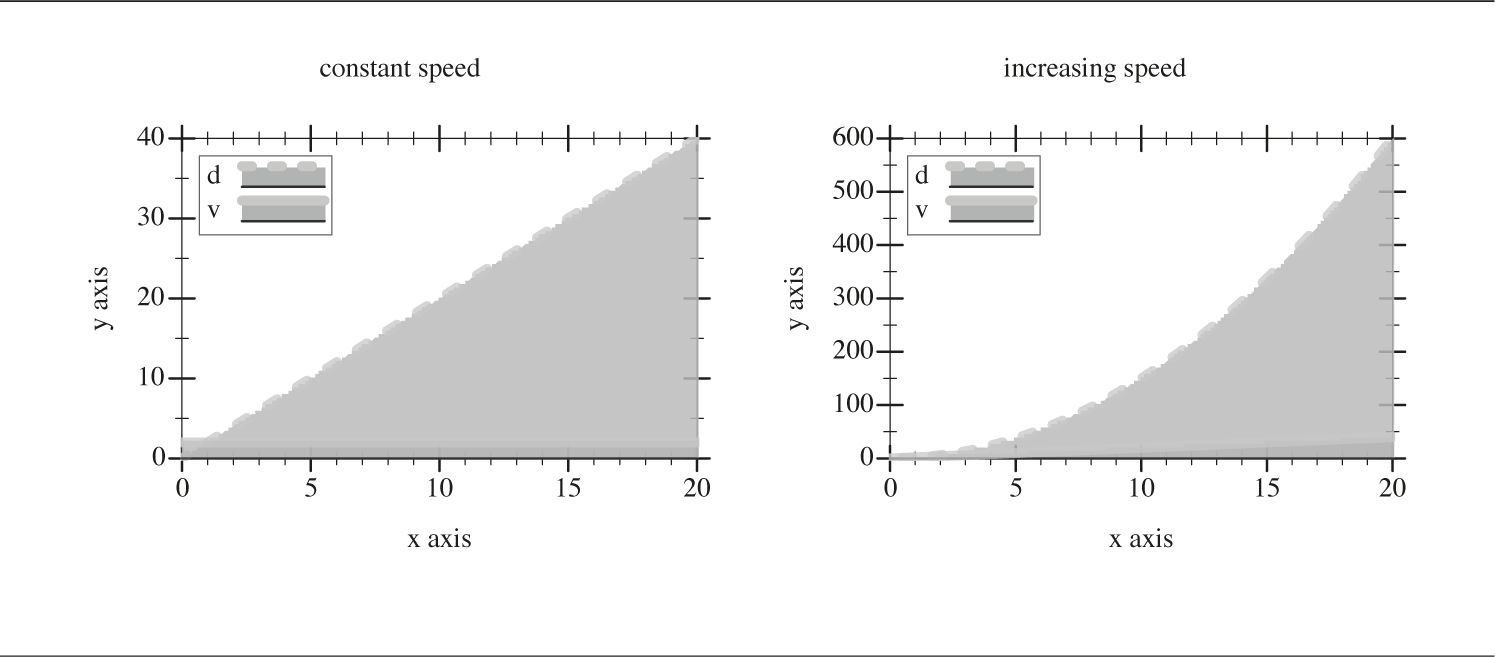
\includegraphics[width=0.85\textwidth]{images/00625.jpeg}
  \caption{匀速行驶与加速行驶中的位移与曲线下面积}
  \label{fig:motion-integral}
\end{figure}

对于任意复杂的曲线（如图~\ref{fig:integral-sketch} 所示），数学解析积分往往极难甚至不可行。计算机科学通过数值近似算法，将曲边图形切分为成千上万个微小的基础几何图形（如矩形、梯形）并对其求和，从而以极高精度逼近积分面积。

\begin{figure}[htbp]
  \centering
  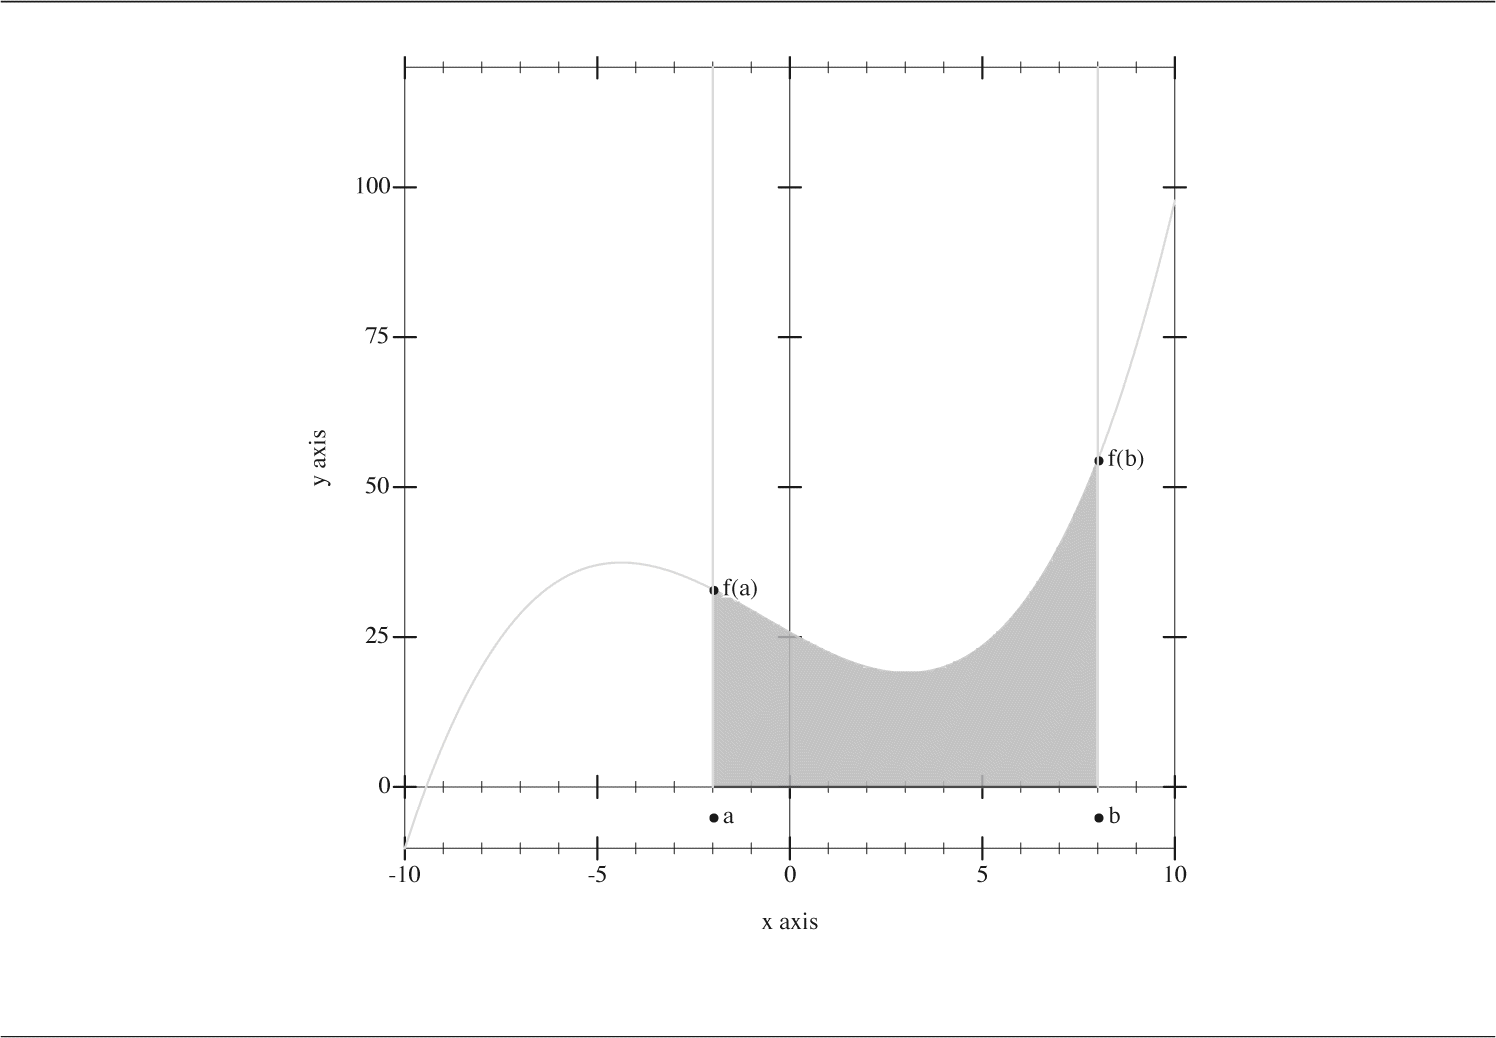
\includegraphics[width=0.75\textwidth]{images/00626.png}
  \caption{在区间 $[a, b]$ 上对函数 $f$ 进行数值积分}
  \label{fig:integral-sketch}
\end{figure}

数值积分函数接收被积函数 $f$ 以及积分区间的左右端点 $a$ 与 $b$：

\begin{lstlisting}[language=BSL]
; [Number -> Number] Number Number -> Number
\end{lstlisting}

图~\ref{fig:generic-integrate} 给出了前三个设计步骤的成果。考虑到浮点近似误差，测试用例统一使用 \code{check-within}，函数头返回 \code{\#i0.0} 显式标明其返回不精确数值。

\begin{figure}[htbp]
  \centering
\begin{lstlisting}[language=BSL]
(define ε 0.1)

; [Number -> Number] Number Number -> Number
; 计算函数 f 在区间 [a, b] 上与 x 轴所围成的面积
; 假设 (< a b) 成立

(check-within (integrate (lambda (x) 20) 12 22) 200 ε)
(check-within (integrate (lambda (x) (* 2 x)) 0 10) 100 ε)
(check-within (integrate (lambda (x) (* 3 (sqr x))) 0 10) 1000 ε)

(define (integrate f a b)
  #i0.0)
\end{lstlisting}
  \caption{通用数值积分函数签名与规范用例}
  \label{fig:generic-integrate}
\end{figure}

\begin{exercise}{开普勒梯形求积法}{458}\label{ex:458}
开普勒（Kepler）提出了一种简便的求积法则：将区间在 $\text{mid} = (a+b)/2$ 处一分为二，计算左侧和右侧两个梯形的面积并相加。梯形面积公式可统一表示为：
\[ \text{Area} = \frac{f(L) + f(R)}{2} \cdot (R - L) \]
设计函数 \code{integrate-kepler}，实现开普勒梯形法。在图~\ref{fig:generic-integrate} 的三个测试用例中，哪一个会出现显著误差？为什么？
\end{exercise}

\begin{exercise}{矩形中点法（黎曼和）}{459}\label{ex:459}
另一种经典数值积分法是将整个区间划分为 $R$ 个等宽的小矩形。每个矩形的宽度为 $W = (b-a)/R$，高度取矩形中点处的函数值 $f(a + (i + 0.5) \cdot W)$。所有矩形面积之和即为积分估计值。
设计函数 \code{integrate-rectangles}。将矩形数量 $R$ 设置为可调常量，观察当 $R$ 逐级提升（如 10, 100, 1000）时，近似精度是如何逼近真实值的。
\end{exercise}

\begin{exercise}{基于分治法的简单数值积分}{460}\label{ex:460}
结合二分折半策略开发函数 \code{integrate-dc}：递归将区间平分，分别计算左右两部分的积分值并相加。当区间跨度小于设定容差时，直接采用开普勒梯形公式。
\end{exercise}

简单的分治求积分（如练习~\ref{ex:460}）存在巨大的计算浪费：对于函数曲线平缓平坦的区域，盲目地深层细分区间不仅毫无必要，而且空耗算力；而对于曲线剧烈振荡震颤的区域（如图~\ref{fig:adaptive-sample} 所示），若不进行足够细致的切分，又会产生致命误差。

\begin{figure}[htbp]
  \centering
  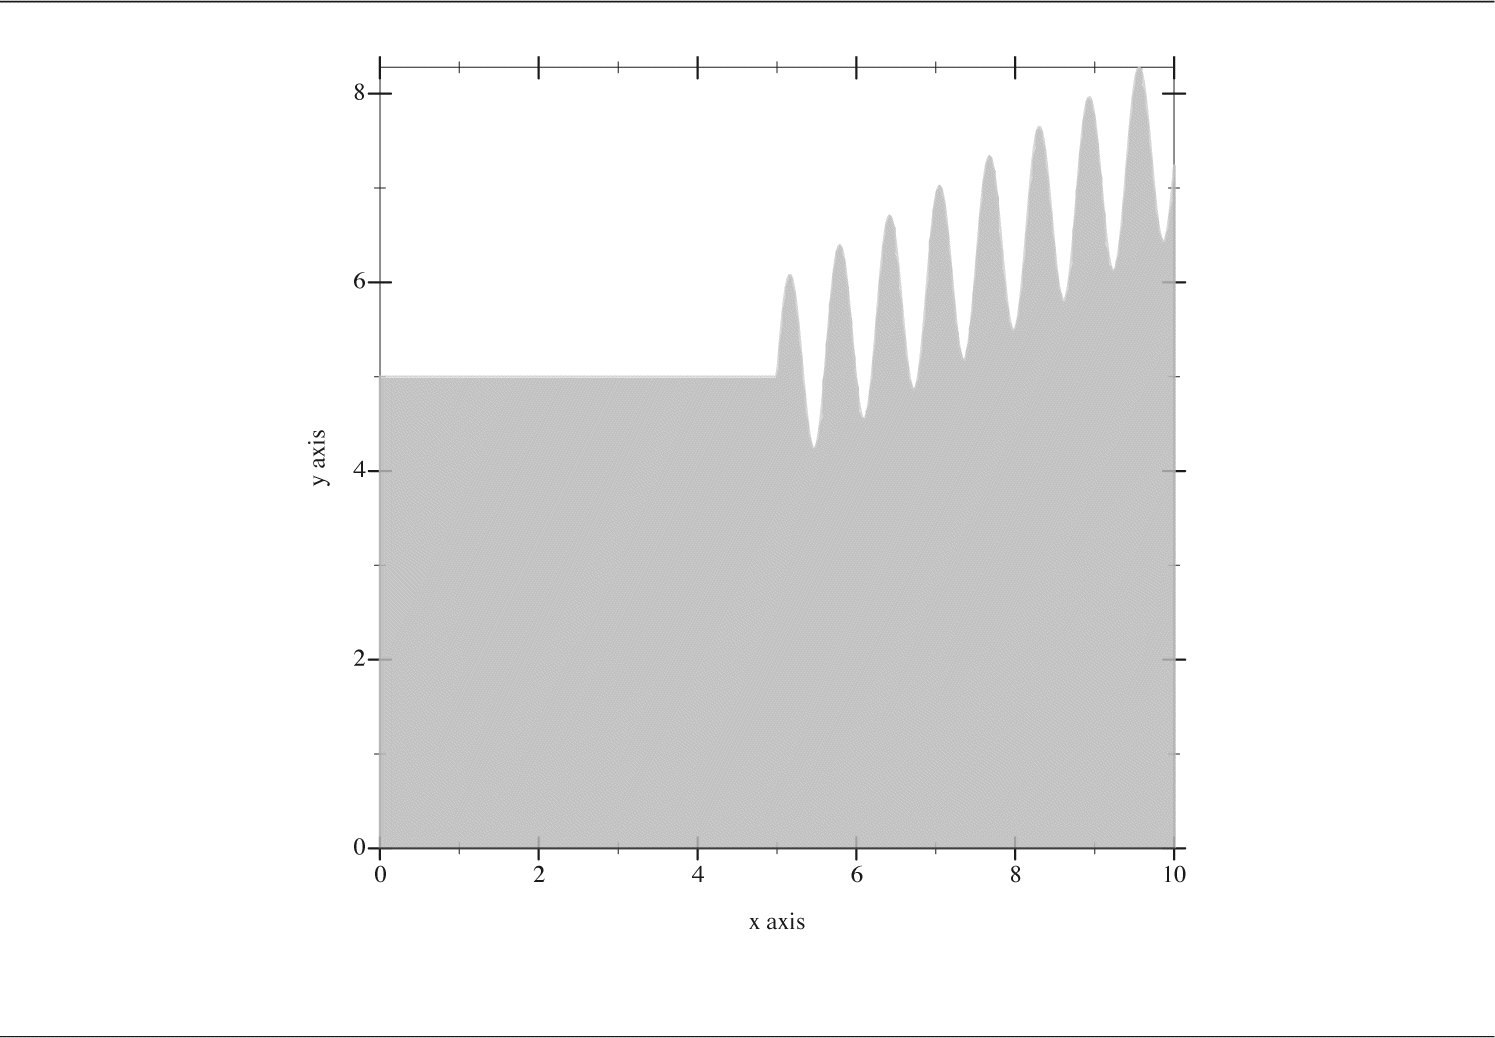
\includegraphics[width=0.75\textwidth]{images/00642.png}
  \caption{自适应积分候选函数：平缓区域与剧烈变动区域共存}
  \label{fig:adaptive-sample}
\end{figure}

为了智能探测函数在当前区域的平缓程度，算法可以计算三个梯形面积：大区间的梯形面积 $A_{\text{single}}$，以及左右两半区间的梯形面积之和 $A_{\text{split}} = A_{\text{left}} + A_{\text{right}}$。若两者的绝对偏差小于容许误差矩形 $\varepsilon \cdot (b - a)$：
\[ |A_{\text{single}} - A_{\text{split}}| \le \varepsilon \cdot (b - a) \]
则可断定当前区间的线性近似已足够优异，直接返回 $A_{\text{split}}$；否则，继续递归分治。这种能根据函数曲线形态\textbf{按需自动分配计算算力}的高级算法，被称为\term{自适应数值积分（adaptive numeric integration）}。

\begin{exercise}{自适应积分算法设计}{461}\label{ex:461}
设计函数 \code{integrate-adaptive}。在平缓区与剧烈变化区对比其实际递归深度与计算开销。为什么说自适应算法是现代计算软件中的必备利器？
\end{exercise}

\section{综合项目：高斯消元法}
\label{sec:28_3}

数学家不仅研究一元非线性方程，还广泛研究多元\term{线性方程组（system of linear equations, SOE）}：
\begin{notebox}[资源物物交换问题]
在物物交换经济中，煤炭（$x$）、石油（$y$）和天然气（$z$）的单位价值由如下三元一次方程组决定：
\begin{align*}
  2x + 2y + 3z &= 10 \\
  2x + 5y + 12z &= 31 \\
  4x + y - 4z &= -7
\end{align*}
\end{notebox}

方程组的解是一组数字 $(x=1, y=1, z=2)$，代入各个方程均能使得等式严格成立。

图~\ref{fig:soe-rep} 确立了该问题域的数据表示：我们用嵌套列表矩阵（\code{Matrix}）来表示方程组，其中每一行是一个方程（\code{Equation}），包含未知数的系数及等式右侧的常数项。

\begin{figure}[htbp]
  \centering
\begin{lstlisting}[language=BSL]
; SOE 是非空矩阵 [Matrix-of Number]
; 约束：对于 (list r1 ... rn)，每行长度 (length ri) 均为 (+ n 1)
; 解释：表示线性方程组

; Equation 是 [List-of Number]
; 约束：Equation 至少包含两个数字
; 解释：若 (list a1 ... an b) 是方程，则 a1 到 an 为系数，b 为等号右侧常数

; Solution 是 [List-of Number]

(define M
  (list (list 2 2  3 10)
        (list 2 5 12 31)
        (list 4 1 -4 -7)))

(define S '(1 1 2)) ; 解向量 (x=1, y=1, z=2)
\end{lstlisting}
  \caption{线性方程组的数据表示}
  \label{fig:soe-rep}
\end{figure}

提取方程左右两侧的工具函数定义如下：
\begin{lstlisting}[language=BSL]
; Equation -> [List-of Number]
(define (lhs e) (reverse (rest (reverse e))))

; Equation -> Number
(define (rhs e) (first (reverse e)))
\end{lstlisting}

\begin{exercise}{解的验证函数 check-solution}{462}\label{ex:462}
设计函数 \code{check-solution}，接收一个 \code{SOE} 和候选 \code{Solution}。当将解代入各方程后所有等式均成立时返回 \code{\#true}，否则返回 \code{\#false}。
\end{exercise}

\term{高斯消元法（Gaussian elimination）}由两阶段构成：第一阶段是\term{三角化（triangulation）}，通过行初等变换将矩形矩阵转化为同解的上三角矩阵；第二阶段是\term{回代求解（back-substitution）}，逐个回代未知数求出最终解。

三角化的生成式思想是：利用第一行方程作为基准（主元行），消去其余各行在第一列上的变量系数，使得除第一行外所有方程的首项系数均变为 0。在我们的样例中，第二行减去第一行得到：
\begin{lstlisting}[language=BSL]
'(0 3 9 21)
\end{lstlisting}
第三行减去第一行的 2 倍得到：
\begin{lstlisting}[language=BSL]
'(0 -3 -10 -27)
\end{lstlisting}
由于首列系数已经全为 0，按照消元惯例我们可以省略开头的 0，从而将剩余部分缩减为一个规模减小一维的子方程组：
\begin{lstlisting}[language=BSL]
'((3 9 21)
  (-3 -10 -27))
\end{lstlisting}
这是一个规模更小的同类子问题！再次执行生成型递归消元，即可获得最终优美的三角形方程组：
\begin{lstlisting}[language=BSL]
'((2 2 3 10)
  (3 9 21)
  (-1 -6))
\end{lstlisting}
此时 $z$ 的值由最后一行一目了然：$-z = -6 \implies z = 2$。

\begin{exercise}{行减法函数 subtract}{465}\label{ex:465}
设计函数 \code{subtract}。它接收两个等长的 \code{Equation}，从第一个方程中减去第二个方程的适当时倍数，使得结果方程首项系数恰为 0，并返回剔除首个 0 之后的剩余列表。
\end{exercise}

\begin{exercise}{初步三角化算法 triangulate}{466}\label{ex:466}
利用 \code{subtract} 设计生成型递归算法 \code{triangulate}，将合法系数的 \code{SOE} 转换为严格上三角矩阵 \code{TM}。
\end{exercise}

在消元过程中，有时会遭遇主元首项系数为 0 的异常情形。数学定理保证：交换方程组中两行的次序不改变其解集。因此，当首项系数为 0 时，可以通过\term{选主元（pivoting，或主元换行）}来寻找合适的主元行。

\begin{exercise}{带主元轮换的稳健三角化}{467}\label{ex:467}
完善 \code{triangulate}：在执行消元前先检查首项系数，若为 0 则通过轮转行列表找到首系数非零的方程置于首位。
\end{exercise}

\begin{exercise}{奇异与无解方程组的错误检测}{468}\label{ex:468}
某些方程组存在多重共线或相互矛盾，导致消元过程中某一列系数全为 0。修改 \code{triangulate}，使其在遇到首项系数全为 0 的退化方程组时显式报错。
\end{exercise}

\begin{exercise}{上三角矩阵的回代求解器 solve}{469}\label{ex:469}
设计函数 \code{solve}，接收上三角方程组 \code{TM}，通过从底向上的回代过程逐个求出变量数值，最终返回解向量列表。
\end{exercise}

\begin{exercise}{完整的高斯消元求解器 gauss}{470}\label{ex:470}
组合 \code{triangulate} 与 \code{solve}，构建完整的 \code{gauss} 函数，实现从一般方程组到解向量的自动化完整求解过程。
\end{exercise}
